\documentclass[11pt,a4paper]{article}

% ------------------------
% Packages
% ------------------------
\usepackage[margin=1in]{geometry}
\usepackage{amsmath,amssymb}
\usepackage{graphicx}
\usepackage{booktabs}
\usepackage[hidelinks]{hyperref}
\usepackage{enumitem}
\usepackage{setspace}
\usepackage{array}
\usepackage{pgfplots}
\usepackage{url}

\pgfplotsset{compat=1.18}



\setstretch{1.15}

% ------------------------
% Title & Author
% ------------------------
\title{\textbf{A Kelly-Based Framework for Risk-Controlled V-Cycle Iterations in Megaprojects}}

\author{
Yanis Benzakour, MSc\\
\small MSc in Complex Systems Engineering, University of Lorraine\\
\small Independent Researcher\\
\small \texttt{yanis.benzakour1@gmail.com}
}

\date{December 24, 2025}

% ------------------------
% Document
% ------------------------
\begin{document}
\maketitle

% ------------------------
% Abstract
% ------------------------
\begin{abstract}
Abstract
Megaprojects frequently face critical decisions during V-cycle iterations: re-iterate to resolve blocking points or proceed despite unresolved issues. This paper proposes a Kelly criterion-inspired framework for optimal resource allocation in such iterations under uncertainty. Project progress is modeled as capital subject to stochastic gains, stagnation, or regression, with outcome probabilities and magnitudes endogenously depending on allocated resources and current engineering maturity. The analysis reveals that classical proportional-risk assumptions lead to degenerate full-commitment policies, inconsistent with observed practice in late-stage megaprojects. By introducing state-dependent regression severity, the model explains why conservative strategies become optimal as project maturity increases. The framework provides a quantitative basis for risk-controlled decision-making in complex systems engineering.


% When I first wrote this paper, I used a multiplicative progression or regression for each iteration. Then I thought to myself, during my past working experience. Most of the iterations are additive. But then I also remembered something. Some iterations can actually be both and I'll give you a very quick example when I was working as a Requirements Engineer.
% Additive example : The customer needs a drawing for a specific Train station. Once this drawing is completed, verified and validated. The project progress goes up additively.
% Multiplicative example : The customer needs a classification for all requirements related to IT. Internally, we found a way to classify these requirements in a single command line. The project progress goes up multiplicatively, right ? Maybe yes, but to keep things simple. I decided in this paper to make the project productivity index (Kt) to go up additively only.

\end{abstract}
\textbf{Keywords:} Kelly Criterion, V-Cycle, Megaprojects, Systems Engineering, Risk Management, Decision Theory

\section{Introduction}

Large-scale engineering projects such as railway systems, aerospace platforms, or energy infrastructures are characterized by high complexity, centralized decision making, and significant uncertainty. Within such projects, the V-cycle is widely used as a systems engineering framework to manage design, integration, verification, and validation activities.

Despite its structured nature, the V-cycle repeatedly confronts project teams with difficult decisions when blocking points emerge. These decisions often involve choosing between re-iterating, consuming time and resources, or proceeding with unresolved requirements, which may result in contractual disputes at project delivery. Although such decisions are frequently guided by expert judgment (often based on experience level and hierarchical level), they are rarely supported by explicit quantitative decision models. As a result, these choices involve risk and can be viewed as strategic gambles.

The decision-making problem addressed in this paper lies at the intersection of systems engineering practice, as formalized in the Systems Engineering Body of Knowledge~\cite{SEBOK}, and risk-optimal allocation theory originating from information theory~\cite{Kelly1956}.


This paper proposes a formal framework for allocating resources to V-cycle iterations under uncertainty, with the objective of maximizing long-term project productivity while controlling the risk of destroying accumulated progress.

%-------------------------------
% Project Progress as Capital
%-------------------------------
\section{Project Progress as Capital}
\label{sec:progress}

We define \emph{project progress} as a state variable representing the fraction of system requirements that have been satisfied and formally validated at a given point in time. Let
\[K_t \in [0,1]\]

denote the project progress at iteration $t$, where $K_t = 0$ corresponds to the start of the project and $K_t = 1$ corresponds to full requirement satisfaction.

Project progress is interpreted as a form of accumulated capital: it embodies the validated design, verified interfaces, and accepted system behaviors upon which subsequent engineering activities depend. As such, progress can be increased through successful iterations, preserved through cautious decision making, or partially destroyed through regression and rework.

In this work, we adopt a multiplicative perspective on the evolution of project progress, reflecting the proportional nature of learning and regression in complex engineering systems. This viewpoint emphasizes that the impact of engineering decisions scales with the amount of progress already accumulated, and that late-stage setbacks may have disproportionately large consequences. The multiplicative assumption is adopted for analytical clarity and to capture lifecycle effects, while recognizing that some engineering activities may produce fixed additive gains. Alternative additive and hybrid formulations are discussed in Section~\ref{sec:discussion}.




%-------------------------------
% Iteration Outcome Model
%-------------------------------
\section{Iteration Outcome Model}
\label{sec:iteration_model}

Each V-cycle iteration involves allocating a fraction $f_t \in [0,1]$ of available project resources and results in an uncertain outcome that affects project progress. The impact of an iteration is modeled through a stochastic variable $\Delta_t \in [-1,1]$, representing the relative effectiveness of the decision under the project context.

The evolution of project progress is governed by the multiplicative update
\begin{equation}
K_{t+1}
=
K_t \left(1 + f_t \Delta_t (1-K_t)\right),
\end{equation}
which ensures that progress remains bounded within $[0,1]$ while capturing diminishing gains near project completion and heightened sensitivity to regression in late project phases.

The random variable $\Delta_t$ admits three qualitative outcomes:
\begin{itemize}
\item $\Delta_t > 0$: net progress, corresponding to the satisfaction of additional system requirements,
\item $\Delta_t = 0$: stagnation, where resources are consumed without measurable progress,
\item $\Delta_t < 0$: regression, reflecting the invalidation or rework of previously validated requirements.
\end{itemize}

This formulation emphasizes that identical iteration decisions may yield different outcomes depending on the stochastic realization of $\Delta_t$ and the current level of project progress. In practice, this reflects the fact that the outcome of a given engineering action is inherently uncertain and depends on the timing of the decision, the surrounding technical environment, and the organizational and system context in which it is executed.


Although engineering decisions are made with rational intent, the outcomes of V-cycle iterations are not always predictable in large-scale systems. The high degree of coupling between subsystems, combined with delayed verification and validation activities, can cause localized changes to produce effects that only materialize much later in the project lifecycle. As a result, decisions that appear beneficial at the time they are taken may later be identified as sources of regression or rework. This motivates modeling iteration outcomes as stochastic rather than deterministic.



%-------------------------------
% Expected Log-Progress Growth
%-------------------------------
\section{Expected Log-Progress Growth}
\label{sec:log_growth}

Following Kelly-type optimization principles, the objective is to maximize the expected logarithmic growth of project progress across iterations. We define
\begin{equation}
G(f_t)
=
\mathbb{E}
\!\left[
\ln\!\left(
\frac{K_{t+1}}{K_t}
\right)
\right],
\end{equation}
which measures the long-term growth rate of project progress induced by allocating a fraction $f_t$ of available resources to an iteration.

Using the multiplicative update introduced in Section~\ref{sec:iteration_model}, the relative progress change can be written as
\begin{equation}
\frac{K_{t+1}}{K_t}
=
1 + f_t \Delta_t (1-K_t),
\end{equation}
so that
\begin{equation}
G(f_t)
=
\mathbb{E}
\!\left[
\ln\!\left(
1 + f_t \Delta_t (1-K_t)
\right)
\right].
\end{equation}

Let $P_+(f_t)$, $P_0(f_t)$, and $P_-(f_t)$ denote the probabilities of progress, stagnation, and regression, respectively. Since stagnation produces no change in project progress, its contribution to logarithmic growth is zero. The expected growth is
\begin{equation}
G(f_t)
=
P_+(f_t)\ln\!\left(1 + f_t \Delta_+ (1-K_t)\right)
+
P_-(f_t)\ln\!\left(1 + f_t \Delta_- (1-K_t)\right).
\end{equation}

A feasibility constraint is imposed to prevent project ruin, requiring that the worst-case outcome preserves strictly positive progress:
\begin{equation}
1 + f_t \Delta_- (1-K_t) > 0.
\end{equation}

%---------
% Reprendre ici
\section{Endogenous Probabilities from Engineering Maturity}

Unlike classical Kelly models, outcome probabilities are endogenous and depend on allocated resources through engineering maturity.

Let $M(f) \in [0,1]$ denote an engineering maturity index defined as a weighted combination of normalized Technology Readiness Level (TRL), System Readiness Level (SRL), interface maturity, and organizational capability.

A simple learning model is:
\[
M(f) = 1 - e^{-\beta f}
\]
where $\beta > 0$ represents learning efficiency.

We define:
\[
P_+(f) = P_+^{\max} M(f)
\]
\[
P_-(f) = P_-^{\min} + (P_-^0 - P_-^{\min}) e^{-\beta f}
\]
\[
P_0(f) = 1 - P_+(f) - P_-(f)
\]

These functions capture diminishing returns, irreducible complexity risk, and stagnation effects.

\begin{figure}[ht]
\centering
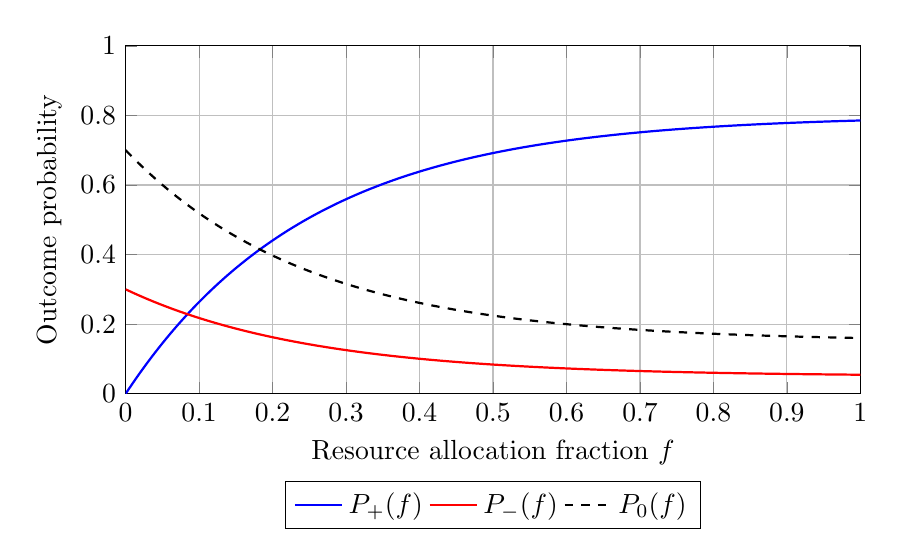
\begin{tikzpicture}
\begin{axis}[
    width=0.9\linewidth,
    height=6cm,
    xmin=0, xmax=1,
    ymin=0, ymax=1,
    xlabel={Resource allocation fraction $f$},
    ylabel={Outcome probability},
    legend style={at={(0.5,-0.25)},anchor=north,legend columns=3},
    grid=both,
    domain=0:1,
    samples=200
]

% ----- Parameters -----
\def\beta{4}
\def\Pplusmax{0.8}
\def\Pminusmin{0.05}
\def\Pminuszero{0.3}

% ----- P+(f) -----
\addplot[thick, blue]
{\Pplusmax*(1-exp(-\beta*x))};
\addlegendentry{$P_+(f)$}

% ----- P-(f) -----
\addplot[thick, red]
{\Pminusmin + (\Pminuszero-\Pminusmin)*exp(-\beta*x)};
\addlegendentry{$P_-(f)$}

% ----- P0(f) -----
\addplot[thick, black, dashed]
{1
 - \Pplusmax*(1-exp(-\beta*x))
 - (\Pminusmin + (\Pminuszero-\Pminusmin)*exp(-\beta*x))};
\addlegendentry{$P_0(f)$}

\end{axis}
\end{tikzpicture}
\caption{Outcome probabilities as functions of allocated resources. Even at full allocation ($f=1$), the probability of regression and stagnation remains strictly positive, reflecting irreducible complexity in large-scale engineering projects.}
\label{fig:outcome-probabilities}
\end{figure}


\section{Optimal Resource Allocation}
\label{sec:optimal_allocation}

The optimal fraction of resources $f^*$ allocated to a V-cycle iteration is obtained by maximizing the expected logarithmic growth of project progress,
\[
G(f) = \mathbb{E}\!\left[\ln\!\left(\frac{K_{t+1}}{K_t}\right)\right],
\]
which yields the first-order condition
\[
\frac{dG}{df} = 0.
\]

This condition balances marginal expected progress gains against marginal regression risk. Under the assumptions of the baseline model, the function $G(f)$ is concave in $f$, ensuring the existence of a unique optimal solution that can be obtained numerically.

However, for the baseline formulation in which iteration outcomes scale proportionally with allocated resources and regression severity is independent of project maturity, numerical evaluation shows that the optimal solution degenerates to the boundary case $f^* = 1$. In other words, the model predicts that allocating all available resources to each iteration is always optimal, regardless of the project’s progress state.

While mathematically consistent with classical Kelly-type models, this result is inconsistent with observed behavior in large-scale engineering projects, where aggressive late-stage decisions often amplify regression and rework rather than accelerate progress.

To mitigate overexposure to such model risk, a fractional Kelly strategy is recommended in practice:
\[
f_{\text{actual}} = \alpha f^*,
\]
with $\alpha \in [0.25, 0.4]$ for large-scale engineering projects. This conservative scaling reflects organizational risk aversion and the high cost of irreversible regression.


\section{Limitations of Proportional Resource Models in Megaprojects}
\label{sec:model_limitations}

The baseline model implicitly assumes that increasing resource allocation improves expected outcomes by proportionally increasing learning and verification capacity. Under this assumption, allocating all available resources ($f=1$) maximizes expected log-growth, as regression impacts remain bounded and scale linearly with effort.

In real-world megaprojects, however, this assumption does not hold. Engineering organizations do not behave as idealized parallel processors: increasing manpower or effort beyond a certain threshold often leads to coordination overload, interface misalignment, and decision amplification. In such contexts, allocating more resources does not guarantee additional progress.

More critically, when a large fraction of the organization converges on an incorrect design decision or implementation strategy, the resulting regression is amplified. Late-stage errors propagate across interfaces, invalidate previously validated requirements, and trigger cascading rework. As a consequence, the magnitude of progress destruction grows with both allocated resources and project maturity.

This observation highlights a fundamental limitation of classical Kelly-type formulations when applied to complex engineering systems: regression risk is not merely proportional but structurally state-dependent. The same decision applied with full organizational commitment can generate modest losses early in the project and catastrophic losses near commissioning.

These considerations motivate the introduction of state-dependent regression mechanisms in the following section, allowing the model to capture the asymmetric and maturity-sensitive nature of risk in large-scale engineering projects.

\section{State-Dependent Regression and Lifecycle Risk}
\label{sec:state_dependent_regression}

To capture the asymmetric impact of late-stage errors in megaprojects, we extend the baseline model by allowing regression severity to depend explicitly on project progress. This modification reflects the empirical observation that regressions occurring late in the lifecycle destroy disproportionately more value than those occurring during early design phases.

Formally, we model the negative outcome magnitude as a state-dependent quantity,
\[
\Delta_-(K_t) < 0,
\]
with $|\Delta_-(K_t)|$ increasing monotonically in $K_t$. Early regressions primarily affect unvalidated design artifacts and are typically localized, whereas late regressions propagate across validated requirements, invalidate verification results, and induce cascading rework.

The project progress update remains multiplicative,
\[
K_{t+1} = K_t \left(1 + f_t \Delta_t\right),
\]
but the distribution of $\Delta_t$ now depends on the project state. In particular, negative outcomes become increasingly destructive as $K_t \to 1$, introducing an explicit lifecycle asymmetry absent from classical Kelly-type formulations.

Under this state-dependent regression structure, the expected log-growth function no longer scales proportionally with project progress. As a result, the optimal resource allocation $f^*(K_t)$ decreases in $K_t$, reflecting the growing fragility of late-stage project progress.

\section{State-Dependent Outcome Probabilities}
\label{sec:state_dependent_probabilities}

In large-scale engineering projects, iteration outcomes are not governed by fixed probabilities. Both empirical evidence and engineering experience indicate that the likelihood of progress or regression depends jointly on the fraction of resources committed and the current maturity of the project. We therefore model iteration outcomes using a state-dependent distribution
\[
P(\Delta_t \mid f_t, K_t).
\]

Let $\Delta_t \in \{\Delta_+, 0, \Delta_-\}$ denote the iteration outcome, corresponding respectively to net progress, stagnation, and regression. The probabilities of these outcomes are defined as follows:
\[
P_+(f_t, K_t) = P_+^{\max} \, M(f_t)\,(1-K_t),
\]
\[
P_-(f_t, K_t) = P_-^{\min} + \big(P_-^{\max} - P_-^{\min}\big)\, f_t \, K_t,
\]
\[
P_0(f_t, K_t) = 1 - P_+(f_t, K_t) - P_-(f_t, K_t).
\]

This formulation captures three key features of megaproject dynamics. First, opportunities for net progress diminish as the project approaches completion, reflecting the decreasing availability of unsatisfied requirements. Second, regression risk increases with both resource commitment and project maturity, modeling organizational convergence and interface coupling effects. Finally, stagnation emerges endogenously when neither meaningful progress nor regression occurs.

By allowing outcome probabilities to depend on both $f_t$ and $K_t$, the model departs from classical Kelly-type formulations and explicitly accounts for lifecycle-dependent risk amplification in complex engineering systems.


\section{Discussion}
\label{sec:discussion}

The proposed framework formalizes a central tension in systems engineering decision making: while aggressive re-iteration can accelerate learning, it also exposes the project to regression and stagnation risks that are difficult to anticipate in complex socio-technical systems. By framing V-cycle iterations as stochastic investments in project progress, the model provides a quantitative interpretation of engineering intuitions commonly held by practitioners.

A key theoretical result of the baseline formulation is that, under proportional outcome assumptions, the Kelly-optimal policy degenerates to full resource commitment ($f^* = 1$) at every iteration. Although mathematically consistent, this prediction contrasts with observed behavior in large-scale engineering projects, where late-stage overcommitment often amplifies coordination failures and propagates errors across already validated requirements.

This discrepancy highlights a fundamental limitation of classical Kelly-type models when applied to megaprojects: regression risk is not merely proportional to invested resources but is strongly dependent on project maturity. Late-stage regressions invalidate previously verified requirements and induce cascading rework, making identical decisions qualitatively more dangerous as the project approaches completion.

While the present analysis adopts a multiplicative progress model for analytical clarity, certain classes of V-cycle activities are more accurately represented by additive progress mechanisms. Hybrid additive--multiplicative formulations may therefore offer a richer representation of project dynamics. Additionally, empirical calibration of state-dependent risks remains an important avenue for future work.



\section{Conclusion}

This paper introduced a Kelly-based decision-theoretic framework for resource allocation in V-cycle iterations of complex engineering projects under uncertainty. By interpreting project progress as a form of capital subject to stochastic gains, stagnation, and regression, the framework captures the inherently risky nature of re-iteration decisions in large-scale systems engineering.

A central finding is that proportional-risk formulations yield a degenerate optimal policy in which full resource commitment is always favored. This result, while theoretically sound, fails to reflect the behavior of real-world megaprojects. By recognizing that regression severity increases with project maturity, the framework explains why conservative decision making becomes optimal near commissioning, even when similar actions were beneficial earlier in the project.

The proposed approach remains intentionally abstract and qualitative. Its primary contribution is to demonstrate that V-cycle decision making is context-dependent, and that identical decisions may produce radically different outcomes depending on project maturity. Future work may extend the model through empirical calibration, hybrid progress formulations, and organizational constraints, further bridging the gap between formal decision theory and systems engineering practice.

Rather than departing from the Kelly criterion, this analysis exposes the implicit assumptions required for its applicability and shows that megaprojects violate these assumptions through state-dependent regression and organizational coupling.

Future extensions could integrate digital twin simulations to estimate state-dependent probabilities in real time, enabling adaptive resource allocation in Industry 4.0 environments.


\newpage
\begin{thebibliography}{9}

\bibitem{Kelly1956}
J.~L.~Kelly~Jr.,
\textit{A New Interpretation of Information Rate},
The Bell System Technical Journal,
vol.~35, no.~4, pp.~917--926, 1956.

\bibitem{SEBOK}
INCOSE SEBOK Editorial Board,
\textit{Systems Engineering Body of Knowledge (SEBoK)},
INCOSE,
available at \url{https://www.sebokwiki.org},
accessed January~2025.

\end{thebibliography}


\end{document}
